\subsubsection*{Rede Neural Profunda}

A principal diferença entre uma rede neural artificial e uma rede neural profunda reside na quantidade de camadas. Enquanto a rede neural profunda possui várias camadas de processamento, a rede neural artificial apresenta menos camadas \apud{marti2017aprendizado}{haykin1999neural}.

\begin{figure}[ht]
\centering
\caption{Comparação entre uma rede neural convencional e uma rede neural profunda.}
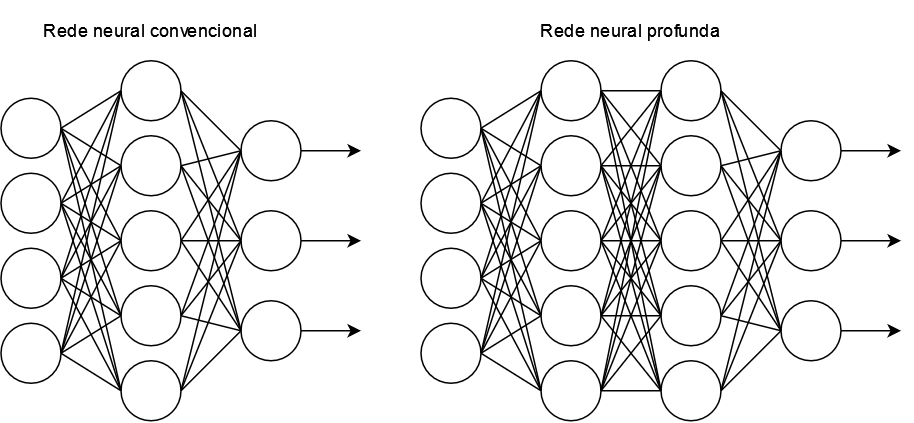
\includegraphics[width=0.8\textwidth]{figures/redes_neurais.png}
\legend{Fonte: Criação própria}
\label{fig:redes_neurais}
\end{figure}